
\documentclass[11pt]{article}
\usepackage[margin=1in]{geometry}
\usepackage{amsmath,amssymb,booktabs,array,longtable}
\usepackage{graphicx}
\usepackage{hyperref}
\usepackage{enumitem}
\usepackage{titlesec}
\usepackage{float}

\begin{document}

\begin{center}
\Large\textbf{Shiv Nadar University Chennai}\\[2mm]
\end{center}

\renewcommand{\arraystretch}{1.4}

\begin{tabular}{|p{3.5cm}|p{8cm}|p{2cm}|}
\hline
Degree \& Branch & B.Tech Artificial Intelligence \& Data Science & Semester V\\ \hline
Subject Code \& Name & CS3807 -- Deep Learning Laboratory & AY: 2026--27\\ \hline
\end{tabular}

\vspace{3mm}

\begin{center}
\Large\textbf{Experiment 1}\\
\large\textbf{Implementation of a Single Layer Perceptron for Binary Classification}
\end{center}

%----------------------------------------------------------

\section*{1. Objective}

The objective of this experiment is to understand the concept of an artificial neuron and implement a Single Layer Perceptron from scratch for binary classification. Students will learn the perceptron learning algorithm, understand the importance of activation functions, visualize the learning process, and evaluate the classifier using a real-world dataset.

%----------------------------------------------------------

\section*{2. Background Theory}

An Artificial Neuron is the fundamental building block of a neural network. It receives one or more input features, multiplies them by corresponding weights, adds a bias term, and applies an activation function to determine the output.

The Single Layer Perceptron is the earliest supervised learning algorithm capable of solving linearly separable binary classification problems.

\subsection*{Mathematical Formulation}

Weighted Sum

\[
z=\mathbf{w}^{T}\mathbf{x}+b
\]

where

\begin{itemize}
\item $\mathbf{x}$ : Input vector
\item $\mathbf{w}$ : Weight vector
\item $b$ : Bias
\item $z$ : Linear combination
\end{itemize}

Prediction

\[
\hat y=f(z)
\]

Weight Update Rule

\[
\mathbf{w}_{new}
=
\mathbf{w}_{old}
+
\eta
(y-\hat y)
\mathbf{x}
\]

Bias Update

\[
b_{new}
=
b_{old}
+
\eta
(y-\hat y)
\]

where $\eta$ denotes the learning rate.

%----------------------------------------------------------

\section*{3. Activation Functions}

An activation function determines the output of a neuron based on the weighted sum of its inputs. It introduces non-linearity, enabling neural networks to learn complex patterns. Although the perceptron uses only the Step Activation Function, modern deep learning models employ differentiable activation functions for efficient optimization through backpropagation.

\subsection*{Step Activation Function}

\[
f(z)=
\begin{cases}
1,&z\ge0\\
0,&z<0
\end{cases}
\]

The Step Activation Function produces a binary output and is therefore suitable only for linearly separable binary classification problems.

\begin{center}
\begin{tabular}{|p{2.5cm}|p{3cm}|p{6cm}|}
\hline
\textbf{Activation} & \textbf{Output Range} & \textbf{Typical Applications}\\
\hline
Step & $\{0,1\}$ & Classical Perceptron\\
\hline
Sigmoid & $(0,1)$ & Binary Classification Output Layer\\
\hline
Tanh & $(-1,1)$ & Hidden Layers (Traditional Networks)\\
\hline
ReLU & $[0,\infty)$ & Hidden Layers in CNNs and MLPs\\
\hline
Leaky ReLU & $(-\infty,\infty)$ & Avoiding Dying ReLU\\
\hline
Softmax & $(0,1)$ & Multi-class Classification Output Layer\\
\hline
\end{tabular}
\end{center}

\textbf{Note:} This experiment uses only the Step Activation Function. The remaining activation functions will be studied in subsequent experiments involving Multilayer Perceptrons and Deep Neural Networks.

%----------------------------------------------------------

\section*{4. Dataset Description}

\textbf{Dataset:} Banknote Authentication Dataset

\textbf{Source:} UCI Machine Learning Repository

\textbf{Download Link:}

\url{https://archive.ics.uci.edu/dataset/267/banknote+authentication}

\begin{center}
\begin{tabular}{|l|l|}
\hline
Instances & 1372\\
\hline
Features & 4 Numerical Features\\
\hline
Classes & 2\\
\hline
Missing Values & None\\
\hline
Task & Binary Classification\\
\hline
\end{tabular}
\end{center}

\textbf{Feature Description}

\begin{itemize}
\item Variance
\item Skewness
\item Curtosis
\item Entropy
\end{itemize}

Target Class

\begin{itemize}
\item 0 -- Authentic Banknote
\item 1 -- Forged Banknote
\end{itemize}

%----------------------------------------------------------

\section*{5. Experimental Procedure}

\textbf{Task 1: Dataset Exploration}

\begin{itemize}
\item Load the dataset.
\item Display the first five samples.
\item Determine dataset dimensions.
\item Identify missing values.
\item Display descriptive statistics.
\end{itemize}

\textbf{Expected Output}

Dataset summary and statistical information.

\vspace{2mm}

\textbf{Task 2: Exploratory Data Analysis}

Generate

\begin{itemize}
\item Histograms
\item Correlation Heatmap
\item Scatter Plot
\item Boxplots
\end{itemize}

\vspace{2mm}

\textbf{Task 3: Data Preprocessing}

\begin{itemize}
\item Normalize all numerical features.
\item Split the dataset into Training (80\%) and Testing (20\%).
\end{itemize}

\vspace{2mm}

\textbf{Task 4: Perceptron Implementation}

Implement from scratch

\begin{itemize}
\item Weight Initialization
\item Bias Initialization
\item Step Activation Function
\item Forward Propagation
\item Perceptron Learning Rule
\end{itemize}

\vspace{2mm}

\textbf{Task 5: Model Training}

Display

\begin{itemize}
\item Epoch Number
\item Misclassified Samples
\item Updated Weights
\item Updated Bias
\end{itemize}

\vspace{2mm}

\textbf{Task 6: Model Evaluation}

Compute

\begin{itemize}
\item Accuracy
\item Precision
\item Recall
\item F1-score
\item Confusion Matrix
\end{itemize}

%----------------------------------------------------------

\section*{6.Source Code}

\url{https://github.com/SamrithaShree/Deep_Learning/tree/main/Lab-1}

%----------------------------------------------------------
\section*{7. Experimental Results}

\subsubsection*{First Five Samples}

\begin{center}
\small
\begin{tabular}{|c|r|r|r|r|c|}
\hline
\textbf{Index} & \textbf{Variance} & \textbf{Skewness} & \textbf{Curtosis} & \textbf{Entropy} & \textbf{Class}\\
\hline
0 & 3.62160 & 8.6661 & -2.8073 & -0.44699 & 0\\
1 & 4.54590 & 8.1674 & -2.4586 & -1.46210 & 0\\
2 & 3.86600 & -2.6383 & 1.9242 & 0.10645 & 0\\
3 & 3.45660 & 9.5228 & -4.0112 & -3.59440 & 0\\
4 & 0.32924 & -4.4552 & 4.5718 & -0.98880 & 0\\
\hline
\end{tabular}
\end{center}

\subsubsection*{Dataset Dimensions}

\begin{itemize}
    \item Number of Instances: \textbf{1372}
    \item Number of Features (including target): \textbf{5}
    \item Dataset Shape: \textbf{(1372, 5)}
\end{itemize}

\subsubsection*{Missing Values}

No missing values were found in the dataset.

\begin{center}
\begin{tabular}{|l|c|}
\hline
\textbf{Feature} & \textbf{Missing Values}\\
\hline
Variance & 0\\
Skewness & 0\\
Curtosis & 0\\
Entropy & 0\\
Class & 0\\
\hline
\end{tabular}
\end{center}

\subsubsection*{Descriptive Statistics}

\begin{center}
\scriptsize
\begin{tabular}{|l|r|r|r|r|r|}
\hline
\textbf{Statistic} & \textbf{Variance} & \textbf{Skewness} & \textbf{Curtosis} & \textbf{Entropy} & \textbf{Class}\\
\hline
Count & 1372.000000 & 1372.000000 & 1372.000000 & 1372.000000 & 1372.000000\\
Mean & 0.433735 & 1.922353 & 1.397627 & -1.191657 & 0.444606\\
Std Dev & 2.842763 & 5.869047 & 4.310030 & 2.101013 & 0.497103\\
Minimum & -7.042100 & -13.773100 & -5.286100 & -8.548200 & 0.000000\\
25\% & -1.773000 & -1.708200 & -1.574975 & -2.413450 & 0.000000\\
50\% (Median) & 0.496180 & 2.319650 & 0.616630 & -0.586650 & 0.000000\\
75\% & 2.821475 & 6.814625 & 3.179250 & 0.394810 & 1.000000\\
Maximum & 6.824800 & 12.951600 & 17.927400 & 2.449500 & 1.000000\\
\hline
\end{tabular}
\end{center}

\subsubsection*{Dataset Information}

\begin{itemize}
    \item Total Entries: \textbf{1372}
    \item Total Columns: \textbf{5}
    \item Numerical Features: \textbf{4}
    \item Target Column: \textbf{Class}
    \item Data Types: \textbf{4 float64, 1 int64}
    \item Memory Usage: \textbf{53.7 KB}
\end{itemize}

\textbf{Inference:} The dataset consists of 1372 samples without any missing values, indicating it is optimal for conducting analysis.
Training models on data without cleaning. All of the input characteristics are numerical and the descrip-
The statistics of various features show different distributions. Therefore Normalizing The Feature is an important task.
Preparation before the training of the perceptron.

\subsubsection*{Data Preprocessing Summary}

The training and testing sets used were normalized by the MinMaxScaler of Python library.

A ratio of 80:20

\begin{itemize}
    \item Training Features: \textbf{(1097, 4)}
    \item Testing Features: \textbf{(275, 4)}
    \item Training Labels: \textbf{(1097,)}
    \item Testing Labels: \textbf{(275,)}
\end{itemize}

%----------------------------------------------------------

\section*{8. Generated Plots with Interpretation}

\subsection*{1. Feature Histograms}

\begin{figure}[htbp]
\centering
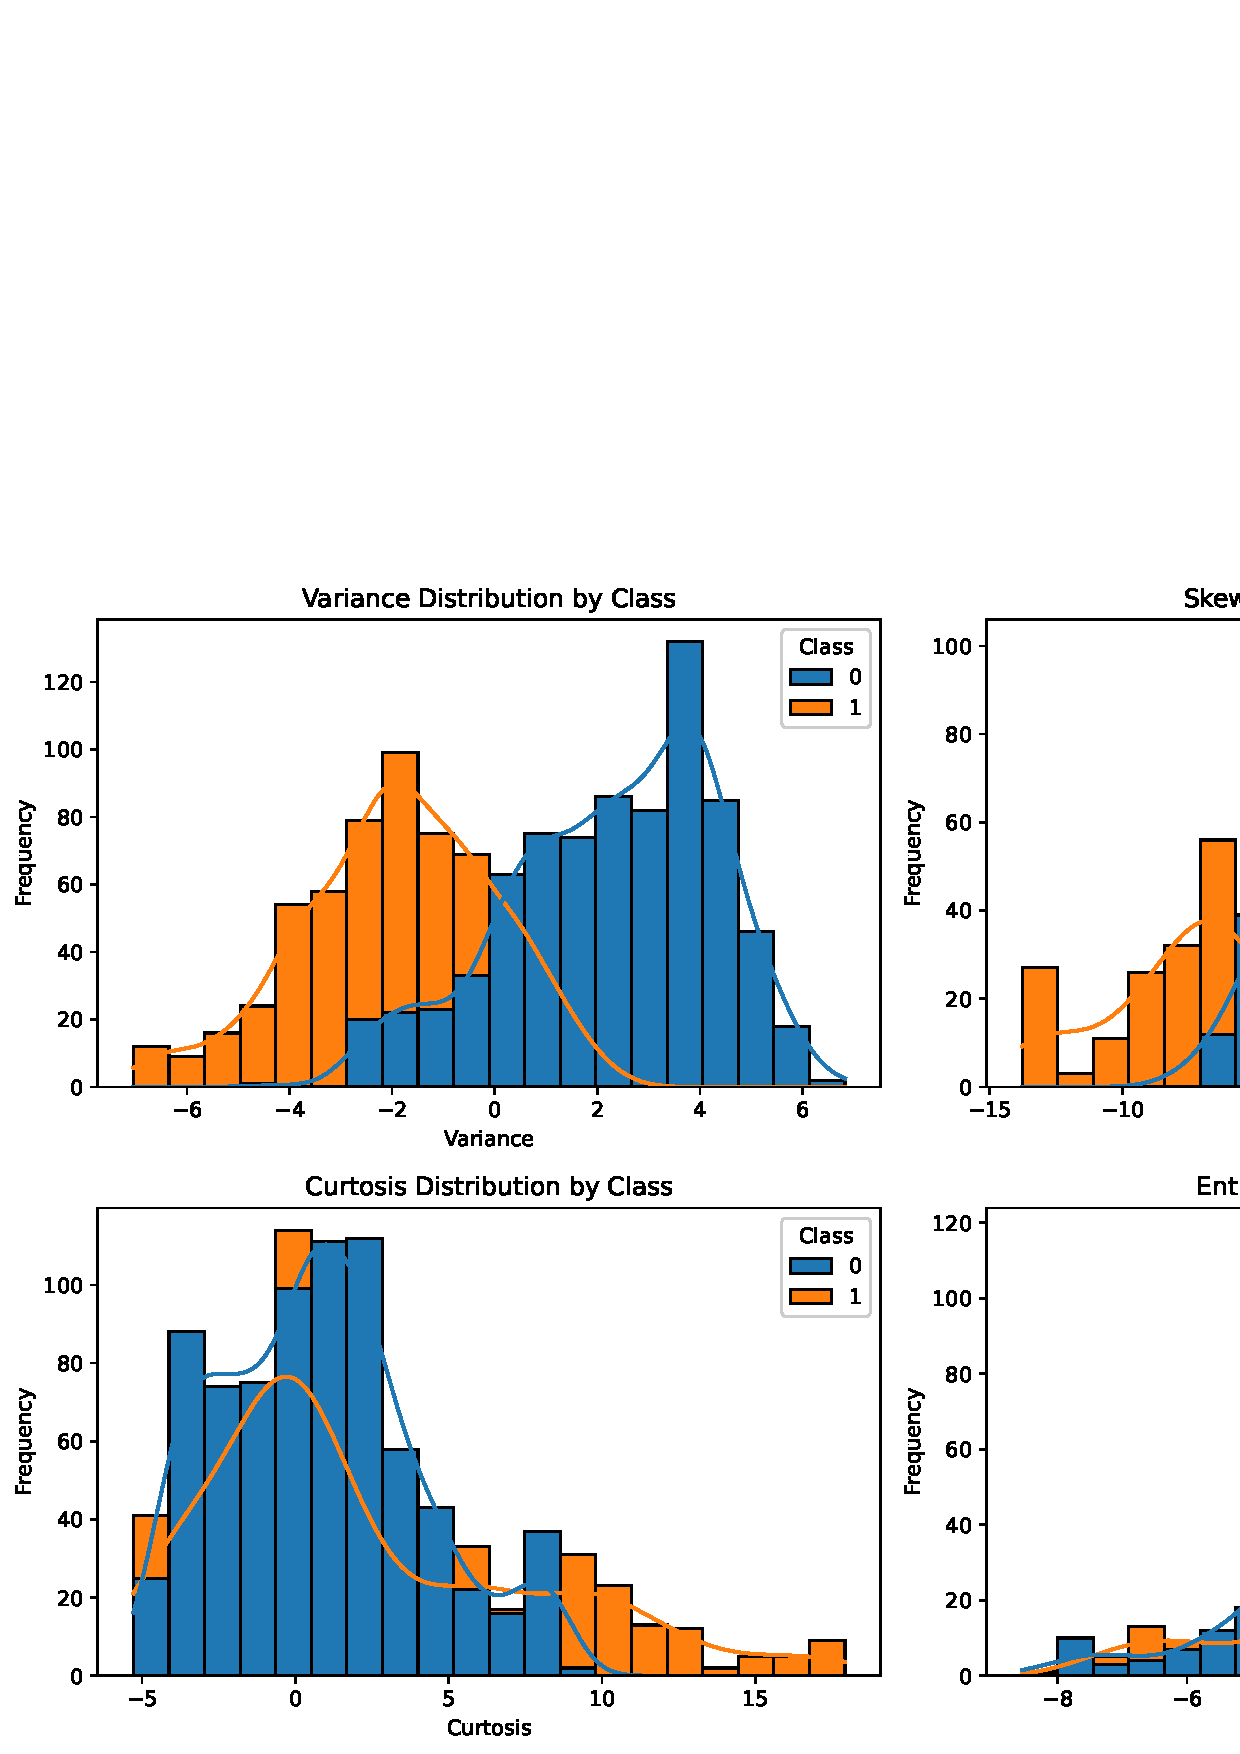
\includegraphics[width=0.85\textwidth]{Feature_Distributions_by_Class.png}
\caption{Feature Histograms for Banknote Authentication Dataset}
\end{figure}

\textbf{Purpose:} Distribution Analysis

\textbf{Interpretation:}
The diagrams show the allocation of each feature for fake and genuine.
Fake Currency Two classes corresponding distributions of most features are slightly skewed.
They possess some degree of uniqueness in distribution and some extreme values, which indicates they are useful for classification.

\vspace{0.5cm}


\subsection*{2. Correlation Heatmap}

\begin{figure}[htbp]
\centering
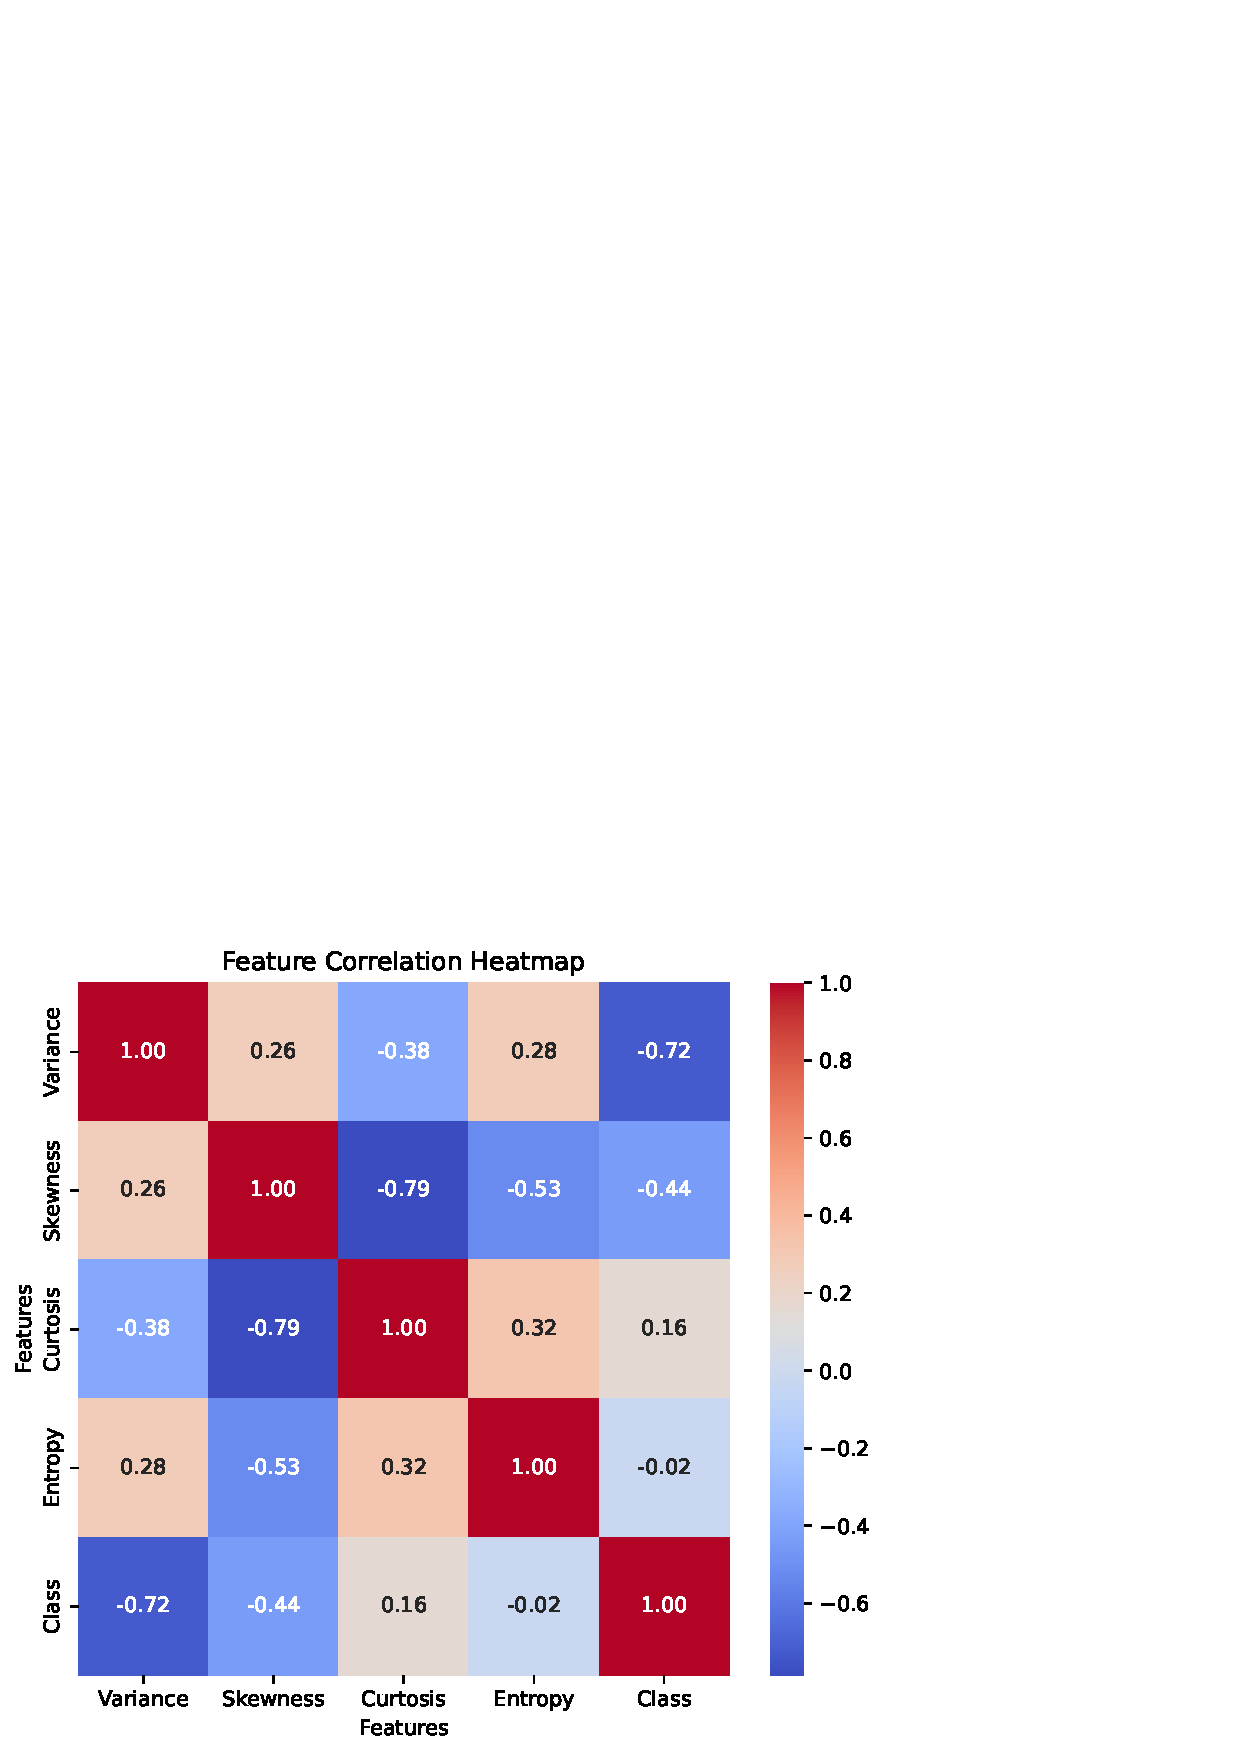
\includegraphics[width=0.75\textwidth]{Correlation_Heatmap.png}
\caption{Correlation Heatmap}
\end{figure}

\textbf{Purpose:} Feature Relationship

\textbf{Interpretation:}
The correlation heatmap shows how input features relate to each other.
Some features show moderate positive or negative correlation no pair is perfectly correlated.
showing that all features contribute useful information.

\vspace{0.5cm}


\subsection*{3. Scatter Plot}

\begin{figure}[htbp]
\centering
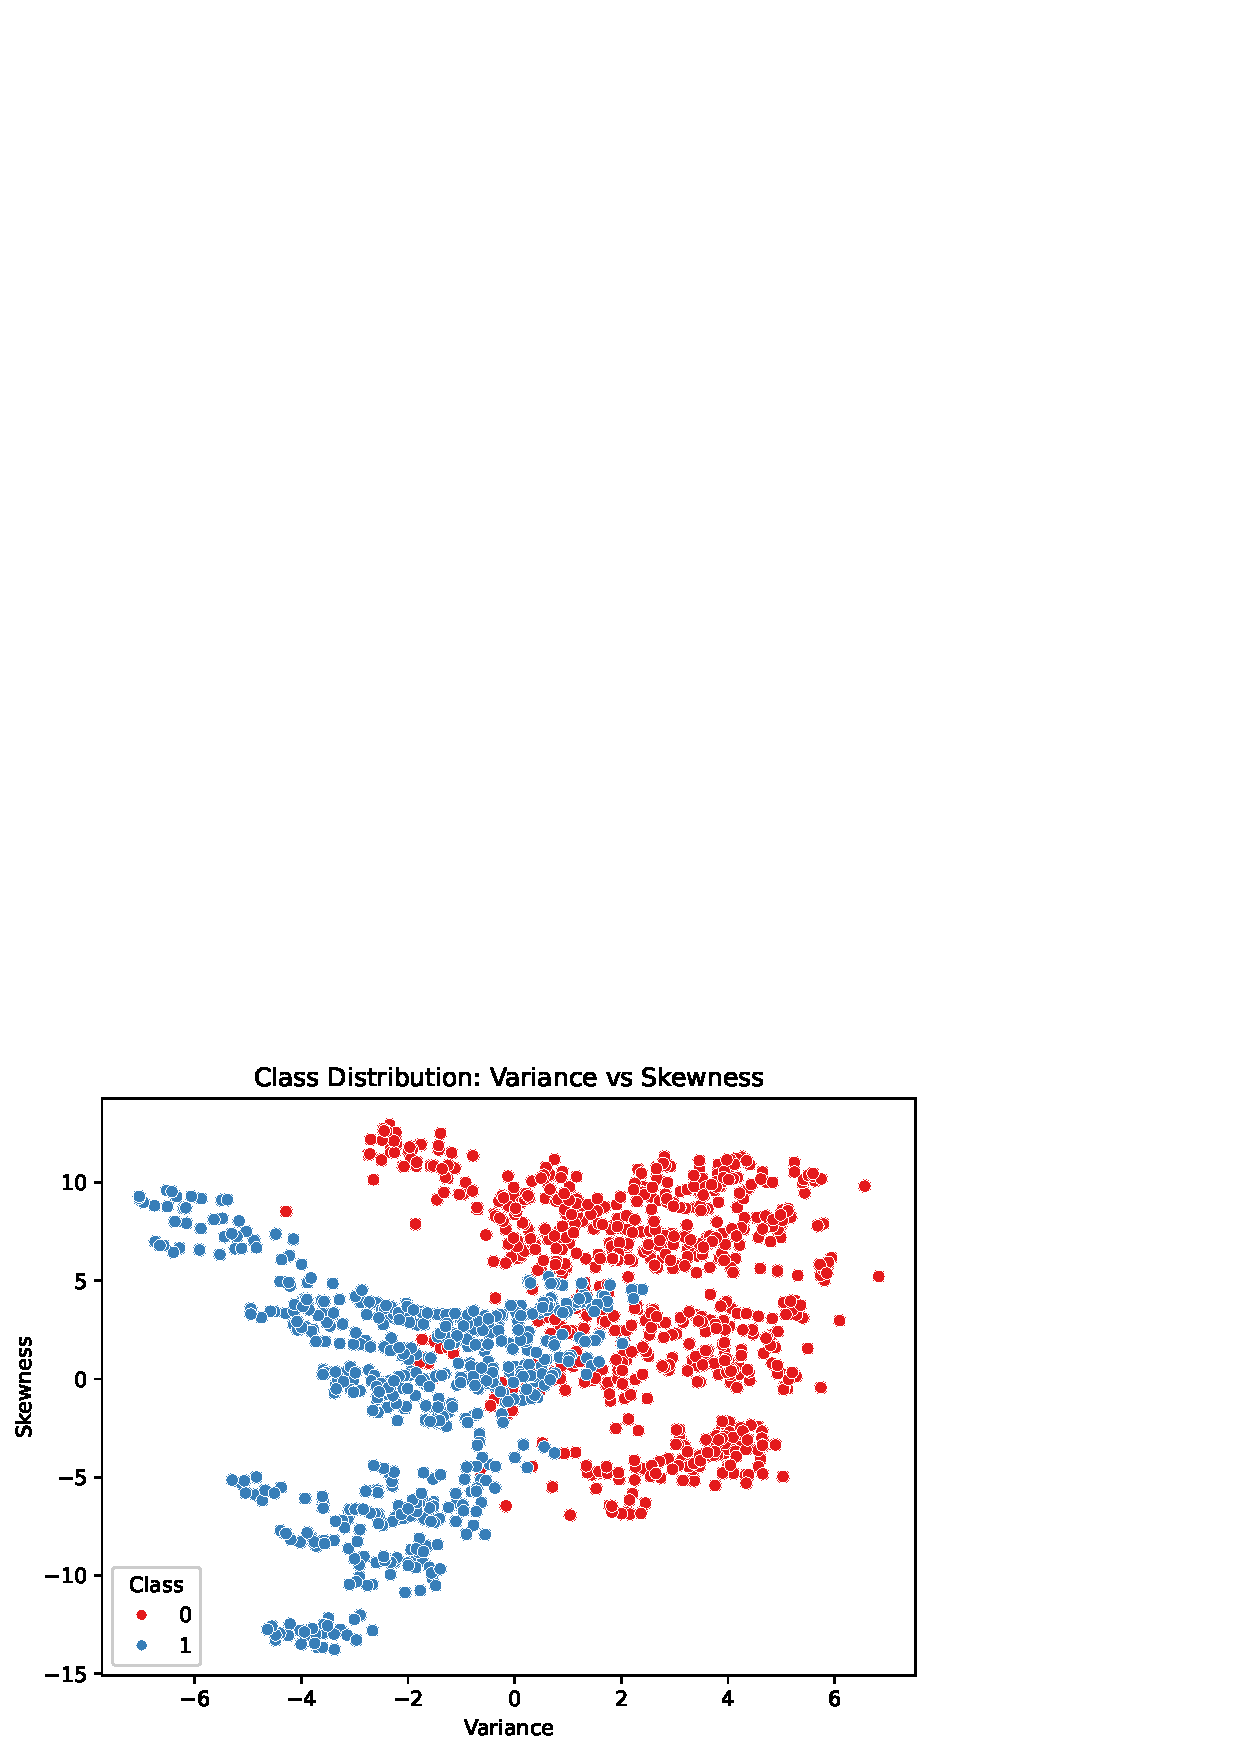
\includegraphics[width=0.75\textwidth]{Scatter_Plots.png}
\caption{Scatter Plot of Variance vs Skewness}
\end{figure}

\textbf{Purpose:} Class Distribution

\textbf{Interpretation:}
Based on the scatter plot, we can interpret that bona fide and counterfeit banknotes are largely different.
The feature space that has been selected, is shown as formable. A linear classifier like the perceptron can achieve this 
Most samples can be classified efficiently.

\vspace{0.5cm}


\subsection*{4. Feature Boxplots}

\begin{figure}[htbp]
\centering
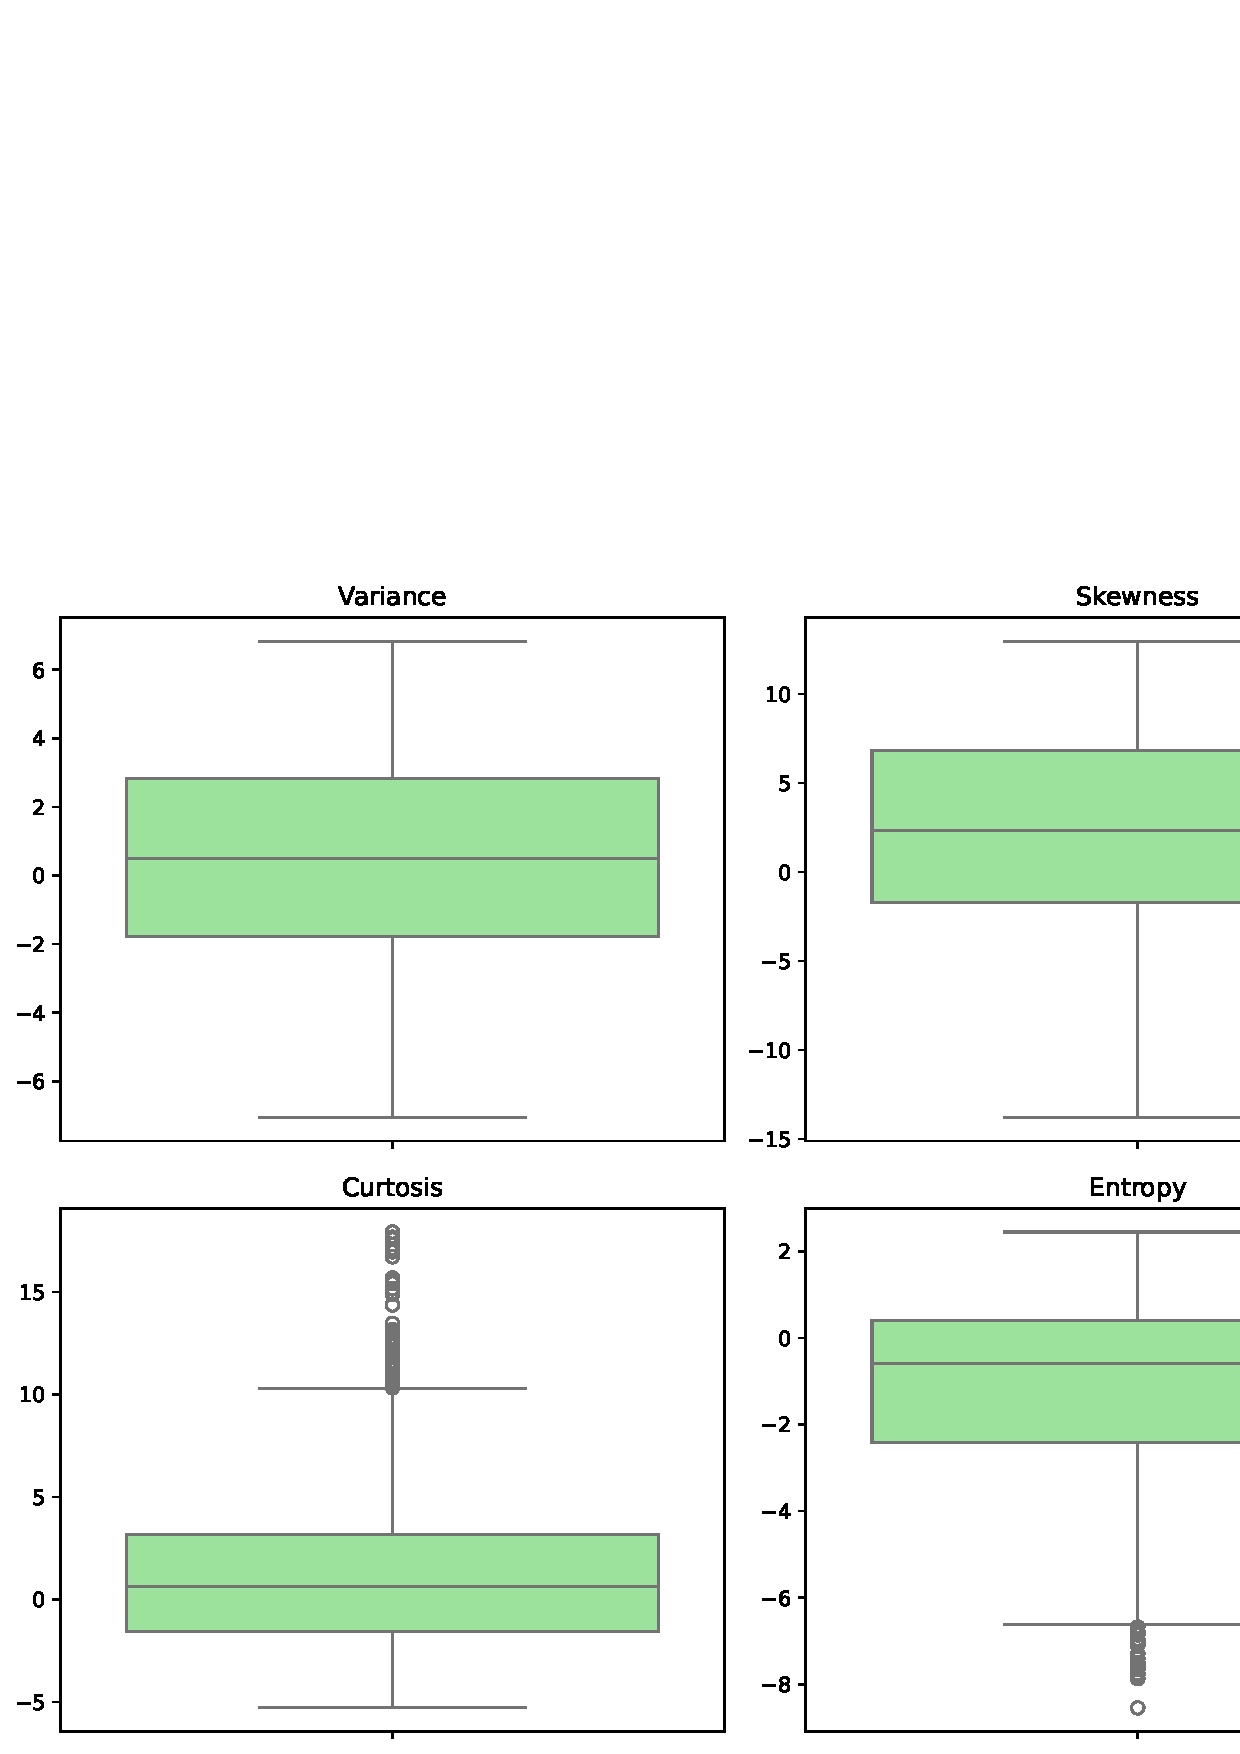
\includegraphics[width=0.75\textwidth]{Feature_Boxplots.png}
\caption{Feature Boxplots}
\end{figure}

\textbf{Purpose:} Distribution Analysis

\textbf{Interpretation:}
The boxplots  give us an idea about the spread of each feature. 
Due to the differences in values among the features normalization is needed.
Trainings.

\vspace{0.5cm}


\subsection*{5. Training Error vs Epoch}

\begin{figure}[htbp]
\centering
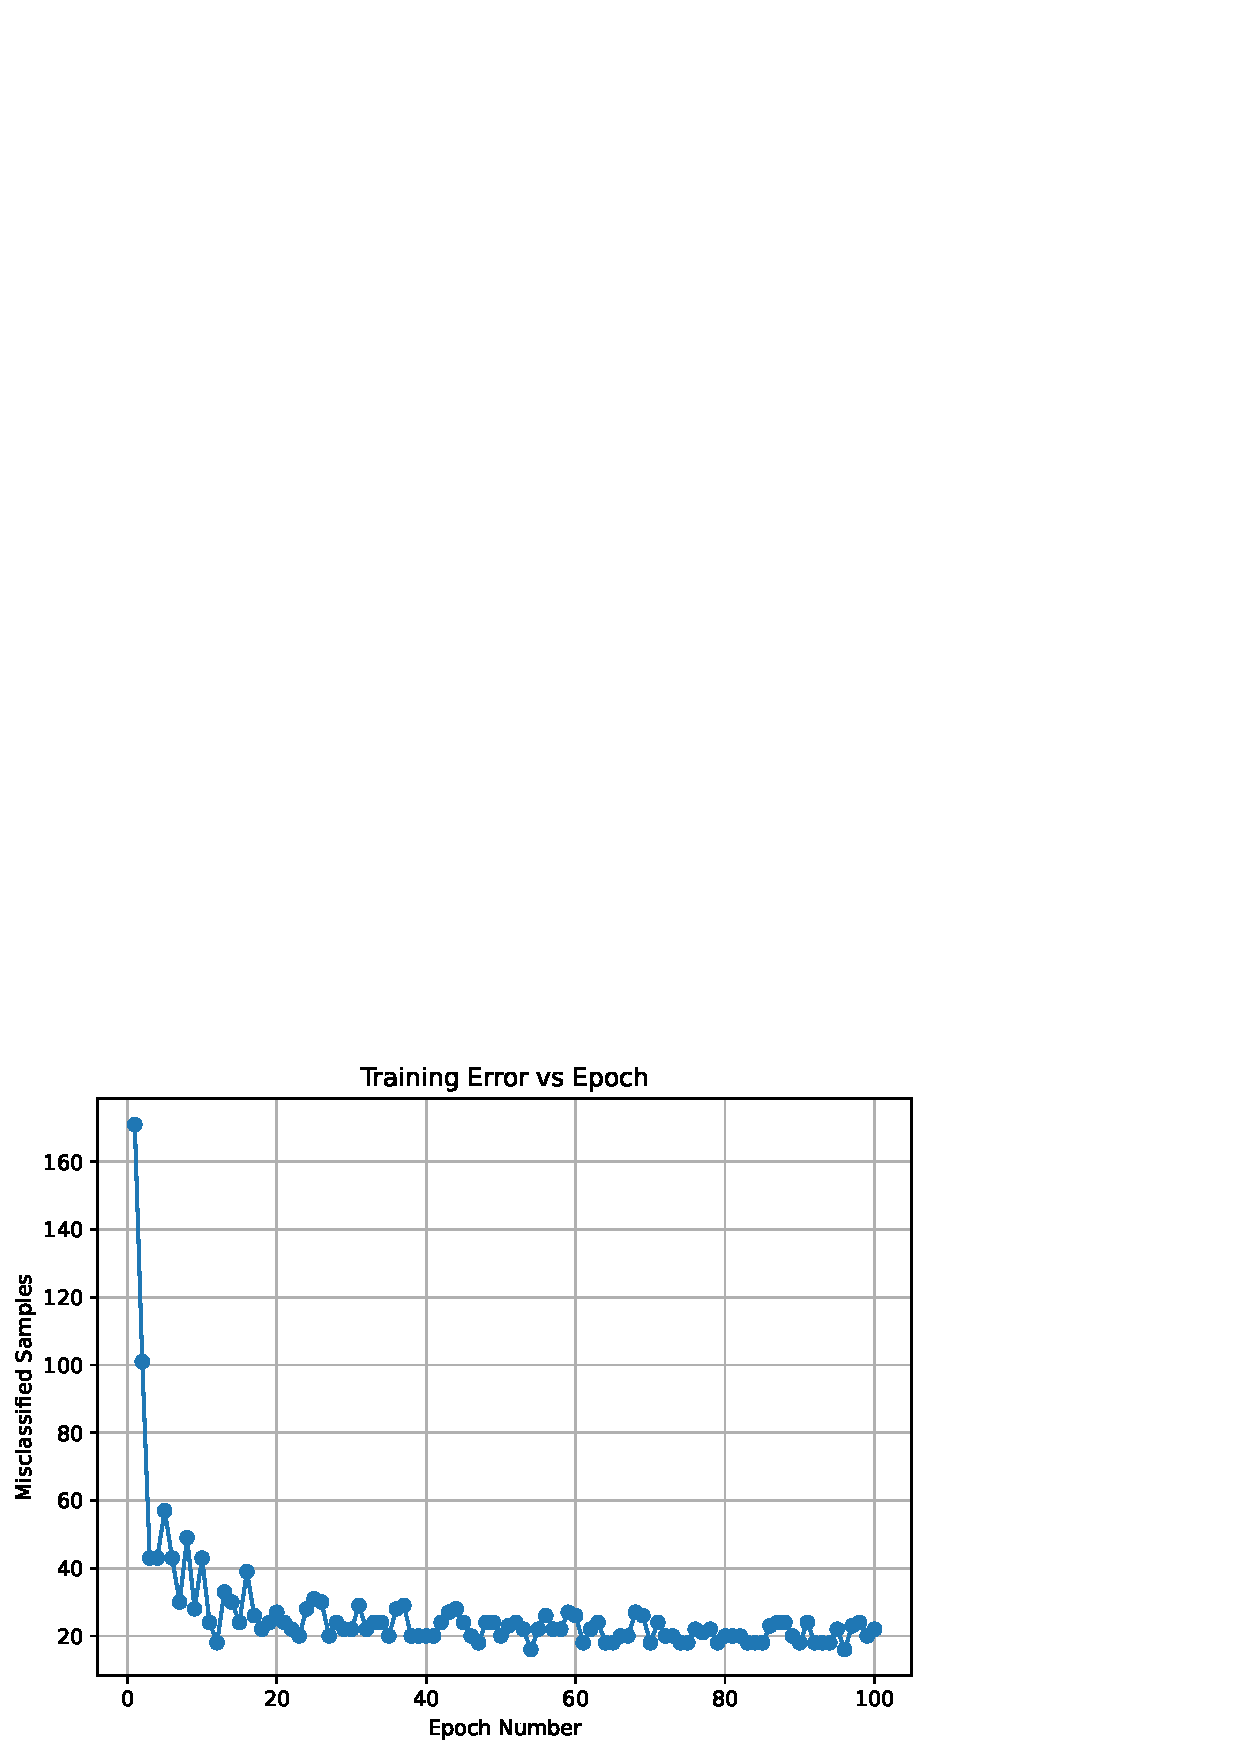
\includegraphics[width=0.75\textwidth]{Training_Error_Vs_Epoch.png}
\caption{Training Error vs Epoch}
\end{figure}

\textbf{Purpose:} Learning Behaviour

\textbf{Interpretation:}
According to the analysis, we see that fewer and fewer samples are misclassified with respect to the number of epochs… stabilizes ultimately. This means that the perceptron manages to find a suitable decision. Limit.

\vspace{0.5cm}


\subsection*{6. Weight Evolution}

\begin{figure}[htbp]
\centering
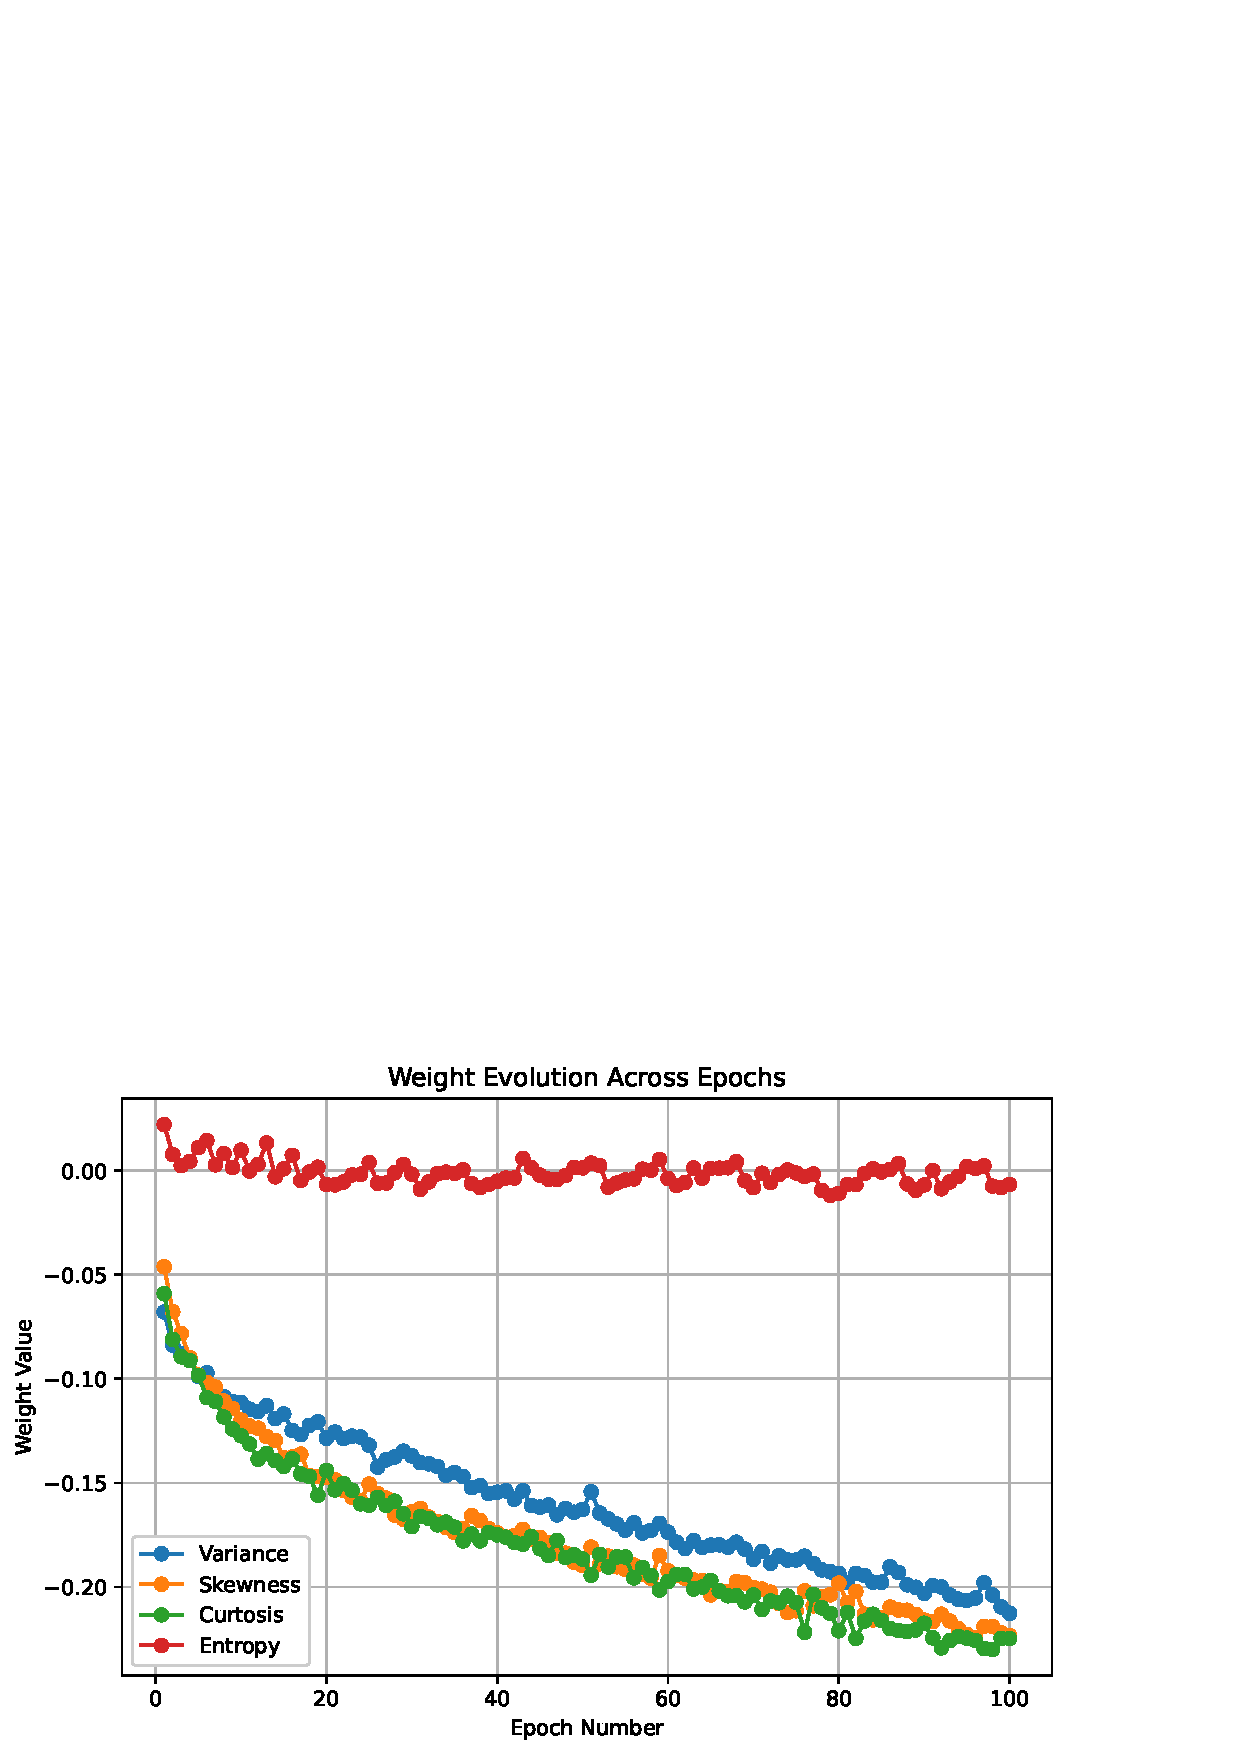
\includegraphics[width=0.75\textwidth]{Weight_Evolution.png}
\caption{Weight Evolution Across Epochs}
\end{figure}

\textbf{Purpose:} Parameter Analysis

\textbf{Interpretation:}
In the interpretative dimension, the feature weights change suddenly in initial epochs and follow through a gradual adjustment.
Values of a parameter improve with training progress. It can be inferred that the learning algorithm is optimal.



\vspace{0.5cm}


\subsection*{7. Bias Evolution}

\begin{figure}[htbp]
\centering
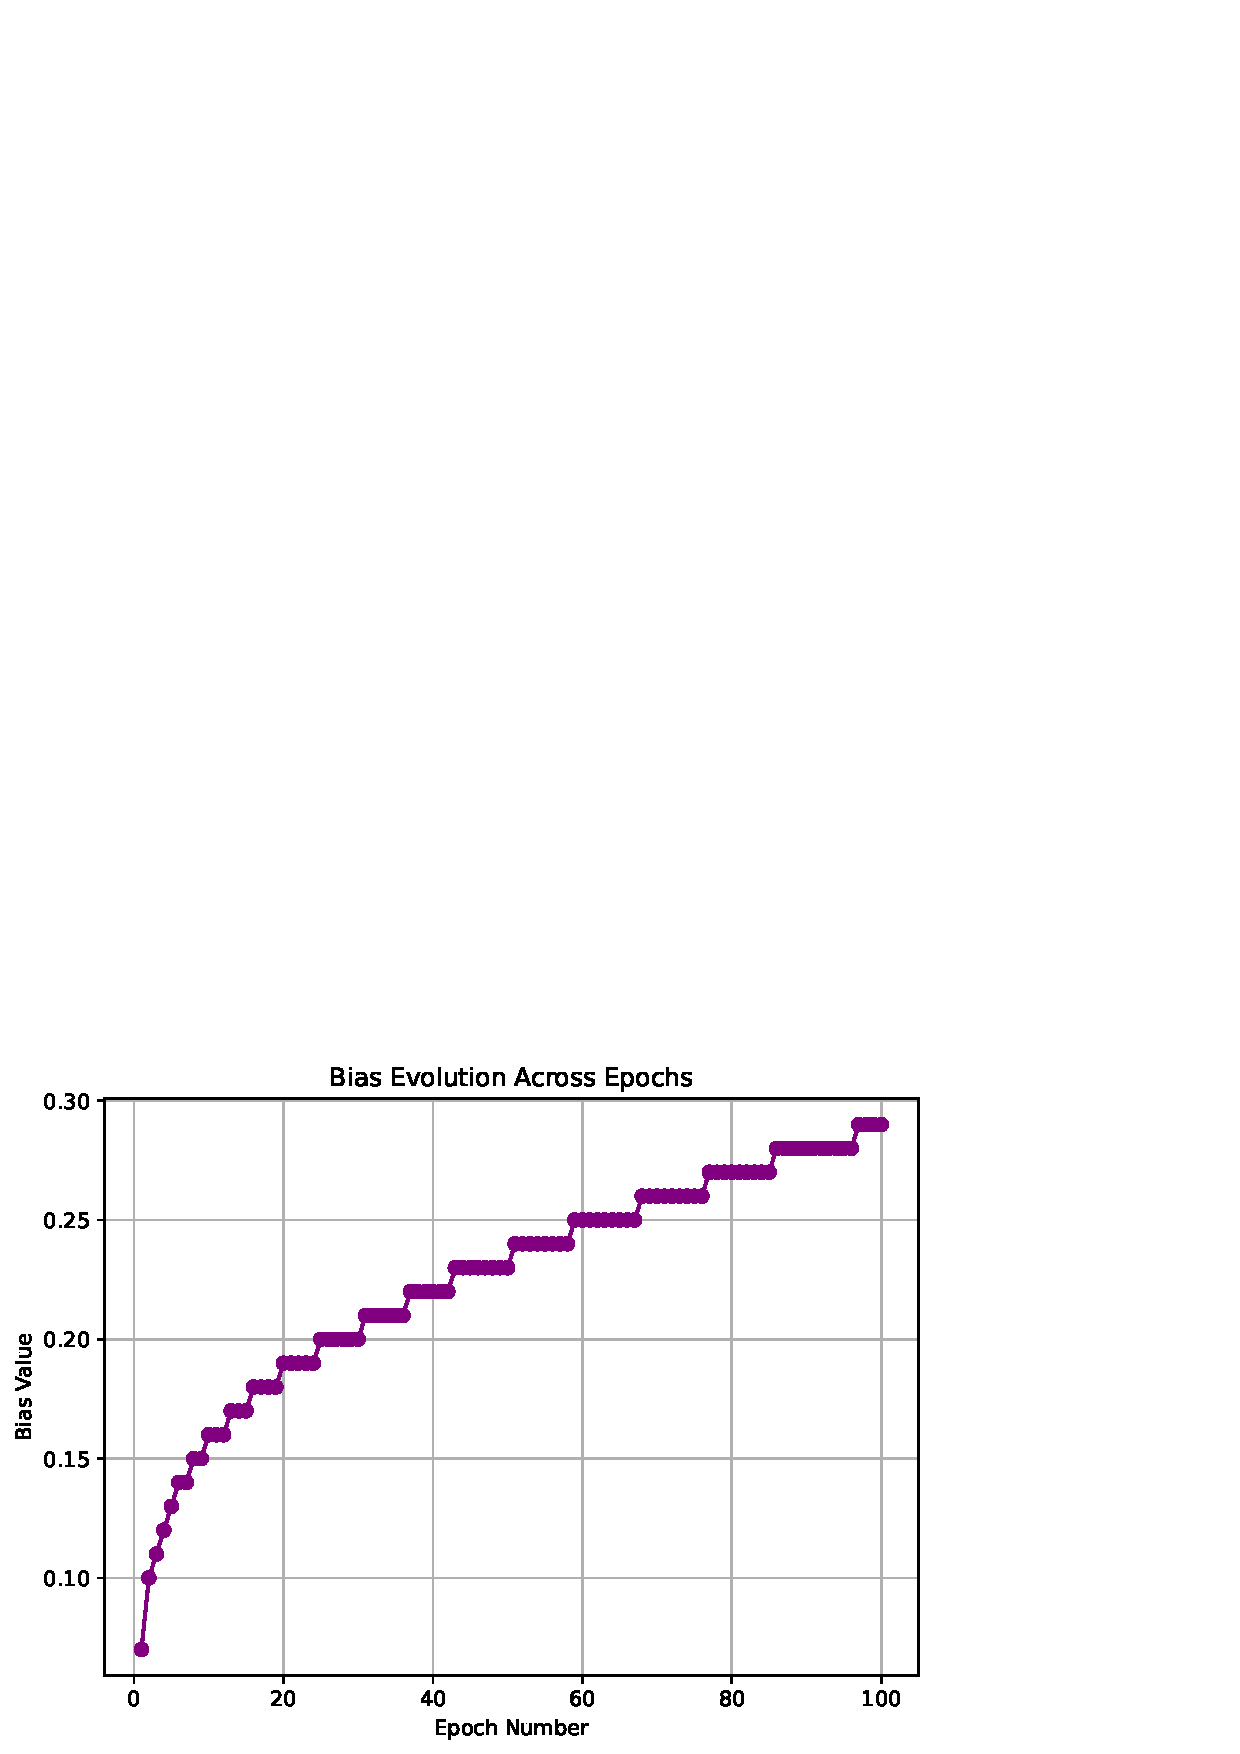
\includegraphics[width=0.75\textwidth]{Bias_Evolution.png}
\caption{Bias Evolution Across Epochs}
\end{figure}

\textbf{Purpose:} Parameter Analysis

\textbf{Interpretation:}
The bias value during training changes to adjust the decision boundary and.
It condusively converges to about 0.29.

\vspace{0.5cm}


\subsection*{8. Confusion Matrix}

\begin{figure}[htbp]
\centering

\includegraphics[width=0.65\textwidth]{Confusion_Matrix.png}
\caption{Confusion Matrix}
\end{figure}

\textbf{Purpose:} Performance Evaluation

\textbf{Interpretation:}
The confusion matrix shows that the perceptron almost classified correctly all test samples, with a misclassification rate of only 3. It has high True Positive (TP) and True TN values that are negative with very few FP and FN resulting in an accuracy of 98.91%.  

\vspace{0.5cm}


\subsection*{9. Learning Rate Comparison}

\begin{figure}[htbp]
\centering
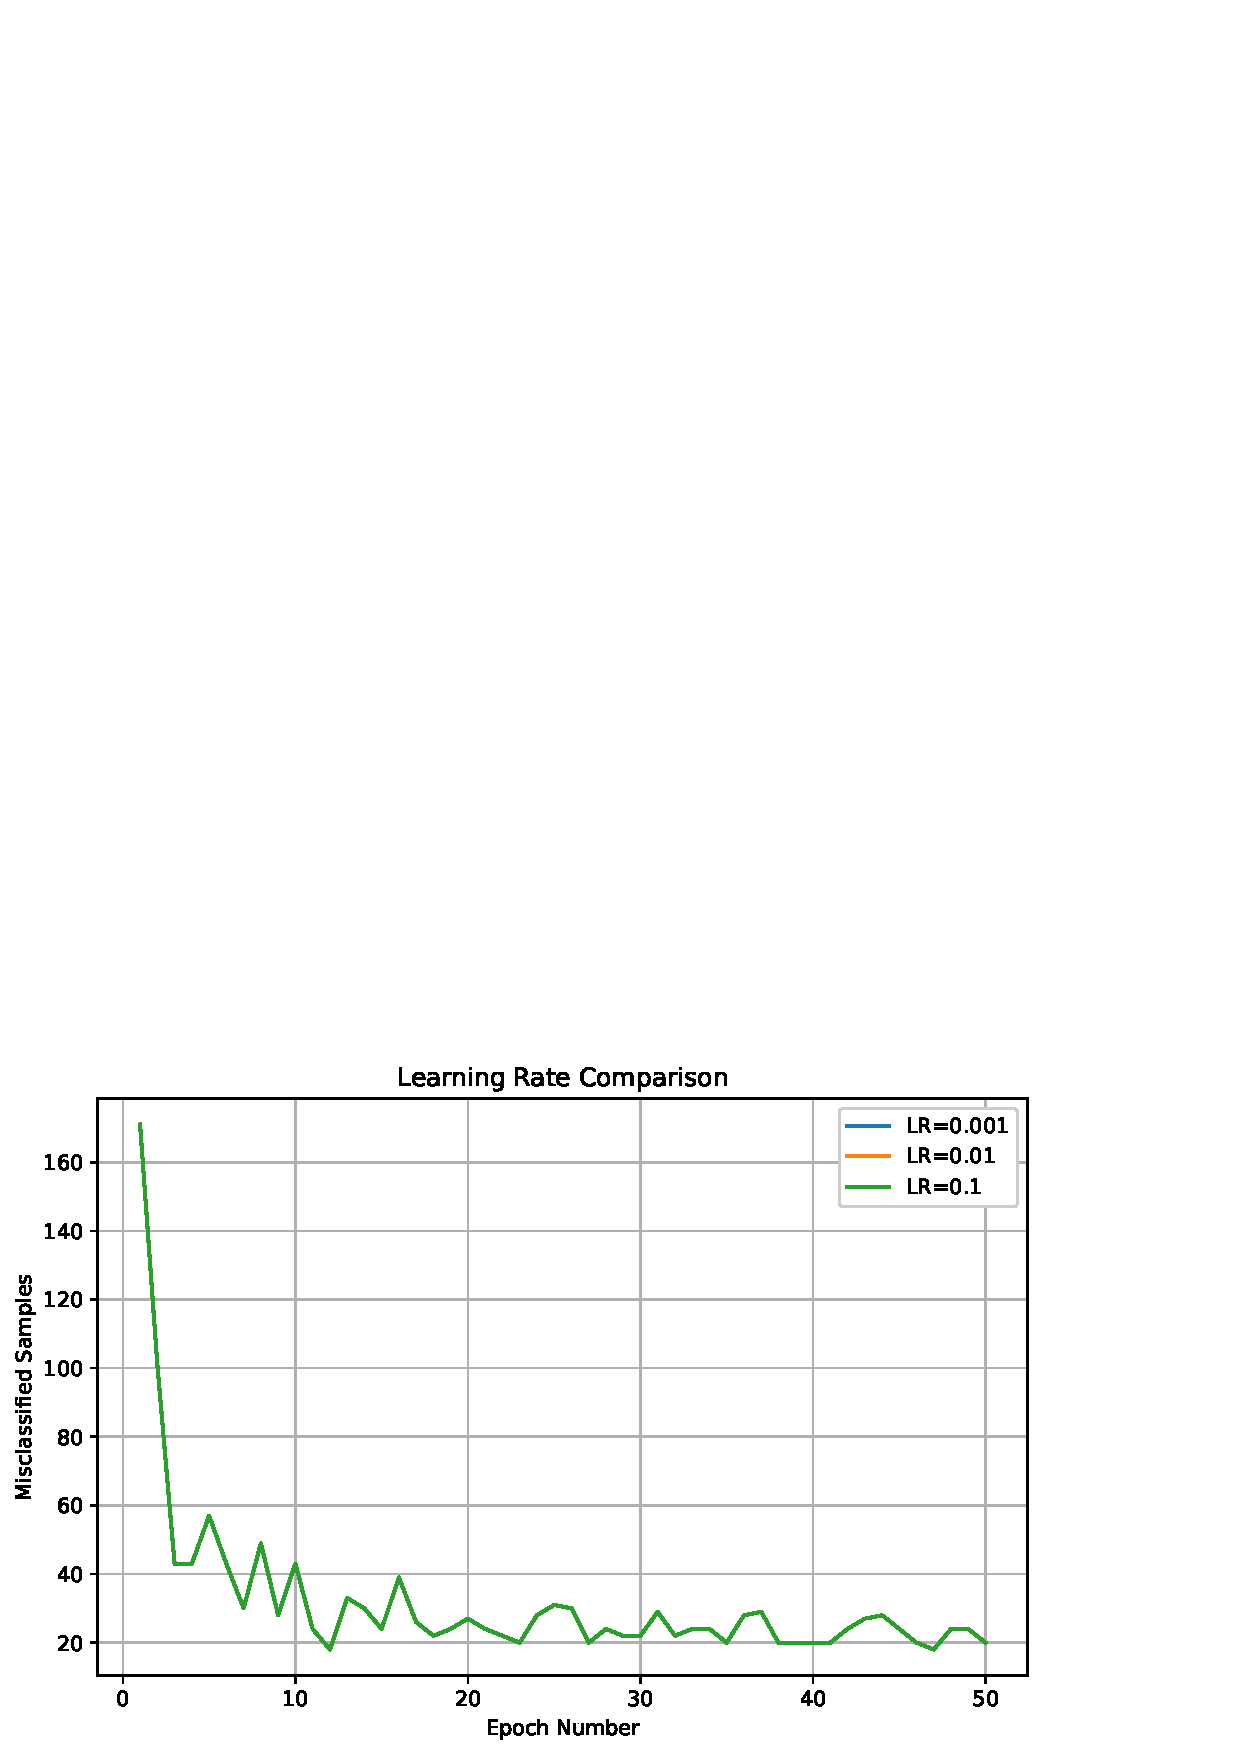
\includegraphics[width=0.75\textwidth]{Learning_Rate_Comparison.png}
\caption{Learning Rate Comparison}
\end{figure}

\textbf{Purpose:} Hyperparameter Study

\textbf{Interpretation:}
The comparison of learning rate shows that larger learning rate converges faster smaller learning rate converges slower a learning rate of 0.01 leads to a good tradeoff between convergence speed and stability for this experiment.


\section*{9. Performance Tables}

\textbf{Training Summary}

\begin{tabular}{|p{6cm}|p{7cm}|}
\hline
Dataset Size &1372\\
\hline
Train/Test Split & 1097 / 275\\
\hline
Learning Rate & 0.01\\
\hline
Epochs & 100\\
\hline
Final Weights & [-0.212646,-0.223446,-0.224733,-0.006686]\\
\hline
Final Bias & 0.29\\
\hline
Accuracy & 98.91\\
\hline
Precision & 99.17\\
\hline
Recall & 98.36\\
\hline
F1-score & 98.77\\
\hline
\end{tabular}

\vspace{3mm}

\textbf{Epoch-wise Learning}


\begin{tabular}{|c|c|c|c|c|}
\hline
\textbf{Epoch} & \textbf{Errors} & \textbf{Weight 1} & \textbf{Weight 2} & \textbf{Bias} \\
\hline
1   & 171 & -0.067924 & -0.046173 & 0.07 \\
25  & 31  & -0.131923 & -0.150585 & 0.20 \\
50  & 20  & -0.162813 & -0.189793 & 0.23 \\
100 & 22  & -0.212646 & -0.223446 & 0.29 \\
\hline
\end{tabular}
%----------------------------------------------------------

\section*{10. Additional Tasks}

\begin{enumerate}[leftmargin=*]

\item \textbf{Comparison of Step and Sigmoid Activation Functions}

\begin{tabular}{|p{4cm}|p{5cm}|p{5cm}|}
\hline
\textbf{Feature} & \textbf{Step Function} & \textbf{Sigmoid Function} \\
\hline
Output Range & 0 or 1 & 0 to 1 \\
\hline
Nature & Discontinuous & Continuous and smooth \\
\hline
Differentiable & No & Yes \\
\hline
Gradient-based Learning & Not Supported & Supported \\
\hline
Applications & Classical Perceptron & Modern Neural Networks \\
\hline
\end{tabular}

\textbf{Discussion:}
The Step Activation Function is not used in modern deep learning because it is non-differentiable almost everywhere and zero gradient, making backpropagation impossible.
The Sigmoid function is differentiable and hence suitable for gradient based optimization.

\vspace{0.4cm}

\item \textbf{Comparison with Scikit-learn's Perceptron}

The custom implementation manually implements the original perceptron learning rule by  weight initialization, forward propagation, step activation and weight updates. Scikit-learn’s implementation is optimized, converges more quickly, supports regularization, early stopping, and a few optimization decisions. Both implementations conduct binary linear-classification, but Scikit-learn is more efficient and practical for the applications.

\vspace{0.4cm}

\item \textbf{Effect of Different Learning Rates}

The perceptron was trained with learning rates 0.001, 0.01 and 0.1.

\begin{itemize}
\item \textbf{0.001:} Slow convergence, need more epochs.
\item \textbf{0.01:} Stable convergence, good classification results.
\item \textbf{0.1:} Faster learning but larger weight updates lead to fluctuations before convergence.
\end{itemize}

Of the three values, a learning rate of 0.01 yielded the best compromise between convergence speed and the stability.

\vspace{0.4cm}

\item \textbf{Why a Single Layer Perceptron Cannot Solve the XOR Problem}

The XOR problem is not linearly separable, meaning that a single straight decision boundary cannot correctly classify all 4 input combinations. Since Single Layer Perceptron can learn only. It cannot solve XOR problem, as it has linear decision boundaries. A Multilayer Perceptron (MLP) non-linear relationship with one or more hidden layers to learn.

\vspace{0.4cm}

\item \textbf{Effect of Feature Normalization on Model Convergence}

Feature normalization is used to scale all the input features to a common range. This prevents features with larger values from dominating the learning process. In this experiment Min-Max normalization resulted in faster convergence, more stable weight updations and better classification performance as compared to un-normalized data.

\vspace{0.4cm}

\item \textbf{Perceptron Learning Behaviour for Logic Gates}

\begin{figure}[H]
\centering
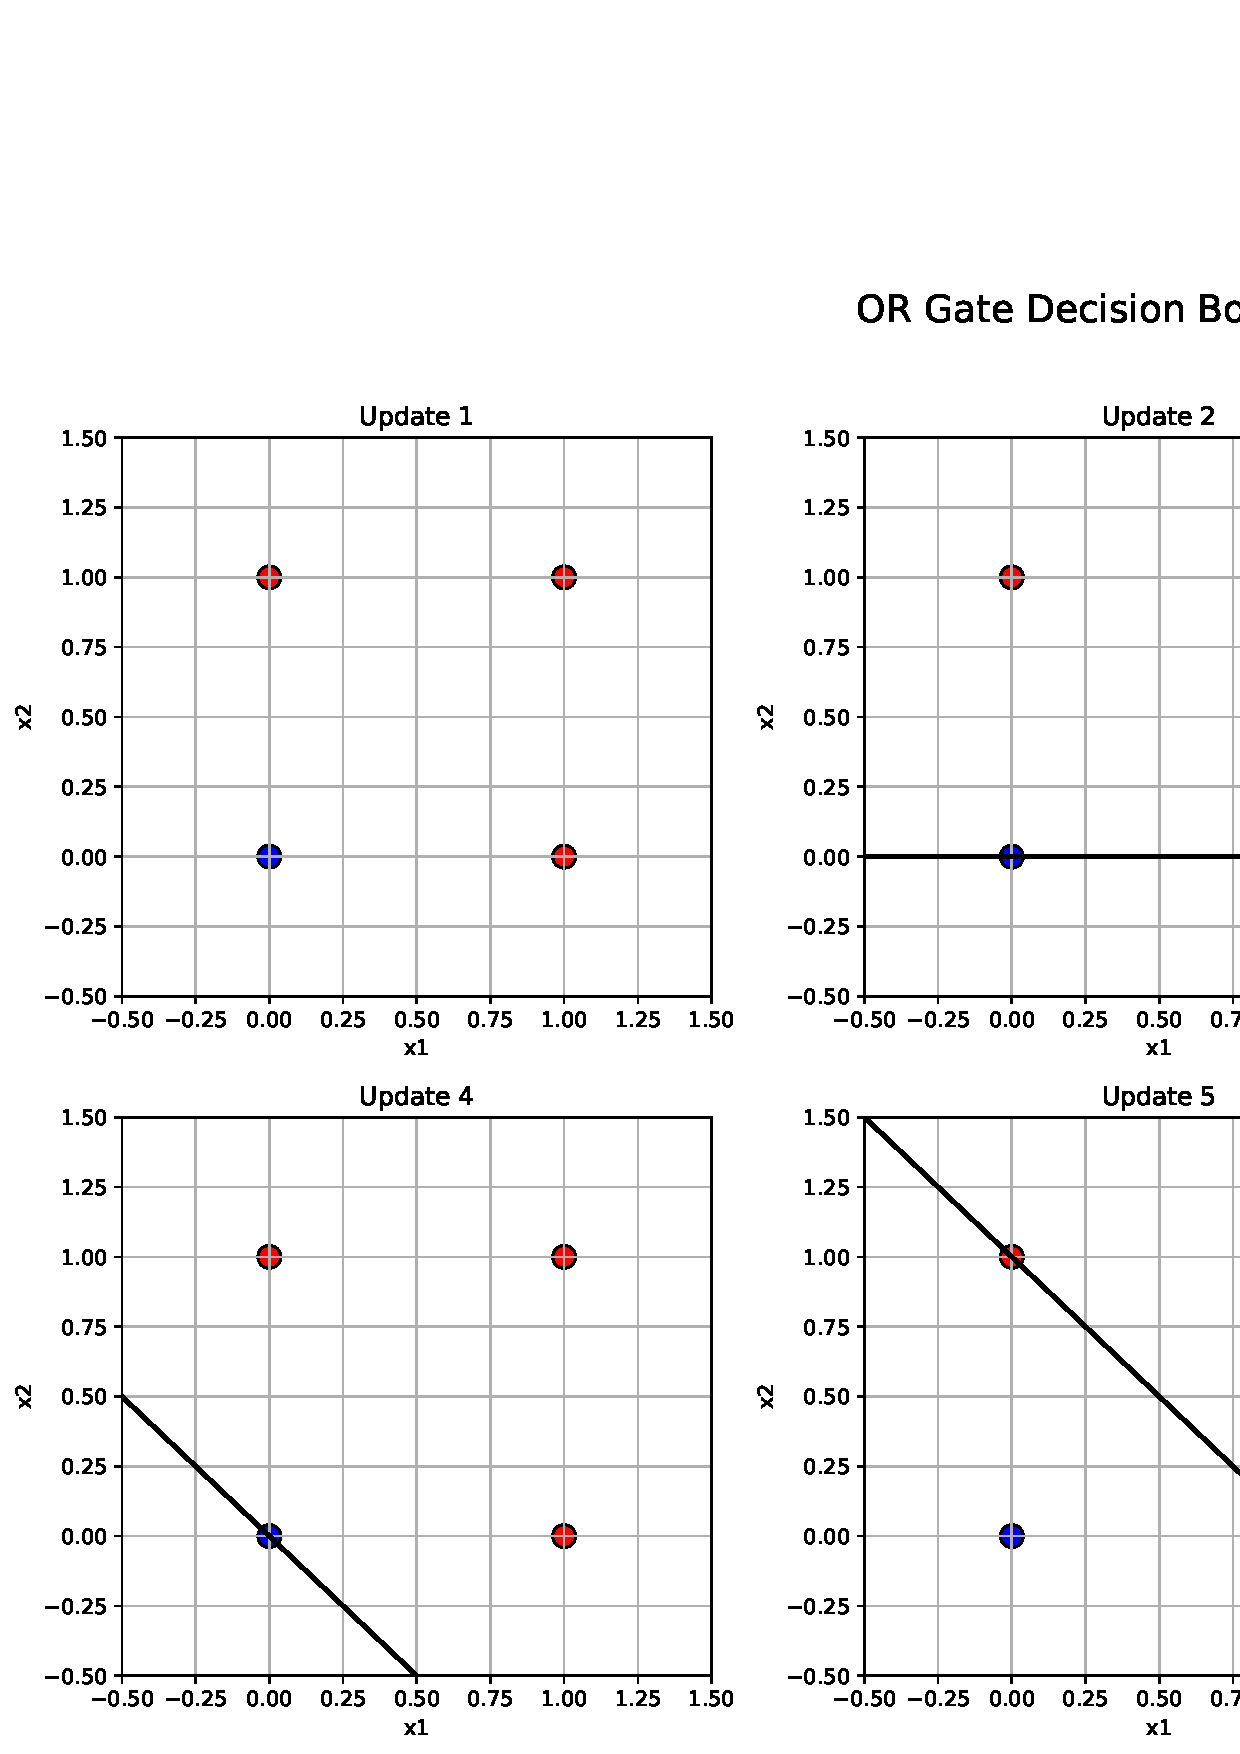
\includegraphics[width=0.95\textwidth]{OR_Gate.png}
\caption{Evolution of the Decision Boundary During Perceptron Learning for the OR Gate}
\end{figure}

\begin{figure}[H]
\centering
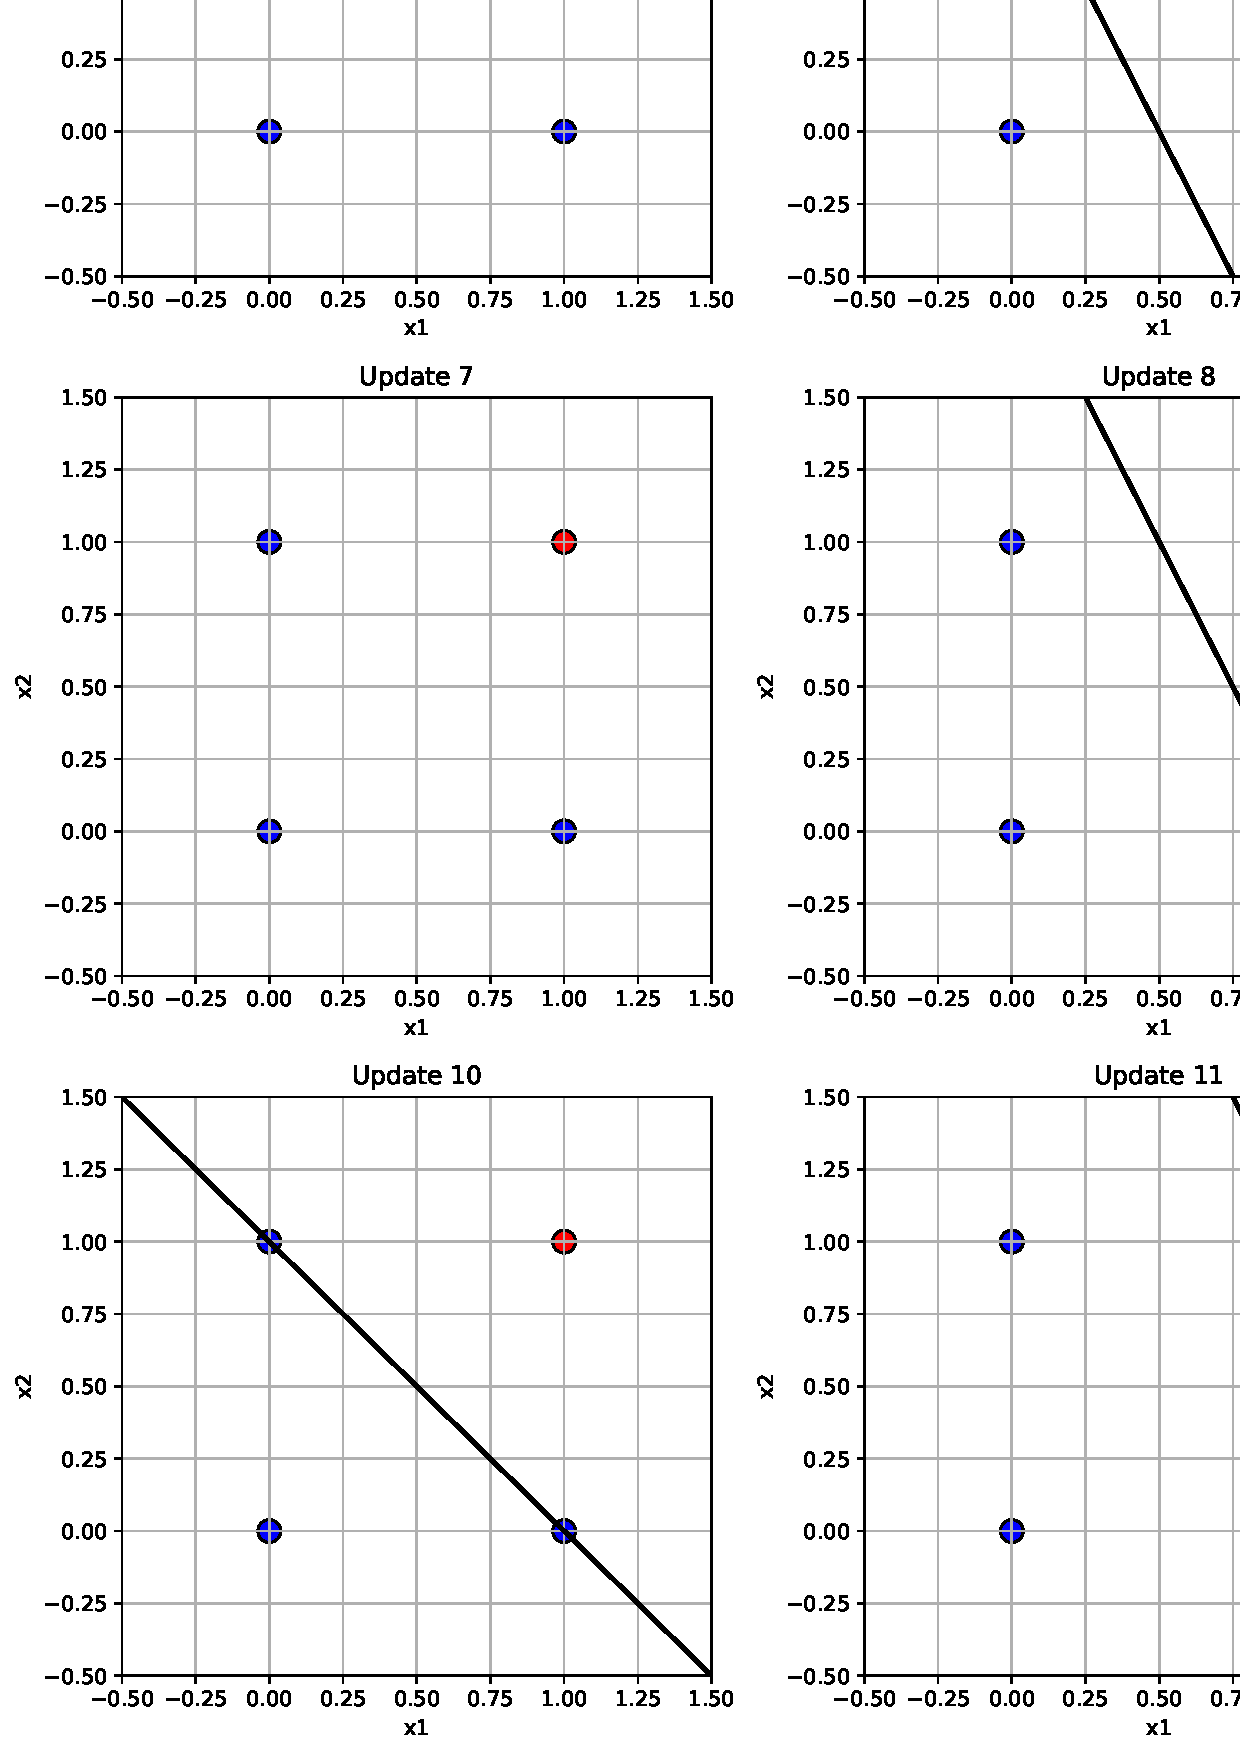
\includegraphics[width=0.95\textwidth]{AND_Gate.png}
\caption{Evolution of the Decision Boundary During Perceptron Learning for the AND Gate}
\end{figure}

\begin{figure}[H]
\centering
\includegraphics[width=0.85\textwidth]{NOT Gate.png}
\caption{Evolution of the Decision Boundary During Perceptron Learning for the NOT Gate}
\end{figure}

\end{enumerate}

% %----------------------------------------------------------

\section*{10. References}

\begin{enumerate}
\item F. Rosenblatt, ``The Perceptron,'' \emph{Psychological Review}, 1958.
\item I. Goodfellow, Y. Bengio and A. Courville, \emph{Deep Learning}, MIT Press, 2016.
\item C. M. Bishop, \emph{Pattern Recognition and Machine Learning}, Springer, 2006.
\item S. Haykin, \emph{Neural Networks and Learning Machines}, Pearson, 2009.
\item UCI Machine Learning Repository -- Banknote Authentication Dataset.
\item Scikit-learn Documentation: Perceptron.
\end{enumerate}

\end{document}

